\documentclass[11pt,a4paper]{report}

\usepackage{amssymb,amsmath,epsfig,float,subfig,hyperref,multicol}
\usepackage{pgfplots}
\usepgfplotslibrary{fillbetween}
\usepackage{xcolor}

\definecolor{SCSUred}{HTML}{CD1041}

\hypersetup{colorlinks=true,linkcolor=SCSUred,urlcolor=SCSUred}

\usepackage{enumerate}
\usepackage{tikz}
\usetikzlibrary{arrows}
\usetikzlibrary{patterns}
\usetikzlibrary{decorations}
%%\usetikzlibrary{intersections}
\usetikzlibrary{matrix}
\usetikzlibrary{snakes}
\usetikzlibrary{calc}
\usetikzlibrary{backgrounds}

\definecolor{linecolor}{HTML}{0074C8}
\definecolor{linecolor2}{HTML}{C80200}

\newcommand{\imagebullet}[1]{\includegraphics[width=0.5cm]{#1}}

\pagestyle{empty}
\setlength{\textwidth}{7in}
\setlength{\textheight}{10in}
\setlength{\oddsidemargin}{-25pt}
\setlength{\evensidemargin}{-25pt}
\setlength{\topmargin}{-50pt}

\usepackage[english]{babel}
\usepackage[utf8]{inputenc}
\usepackage{fancyhdr}
 
%%\pagestyle{fancy}
\renewcommand{\headrulewidth}{0pt}
%%\fancyhf{}
%%\rhead{Share\LaTeX}
%%\lhead{Guides and tutorials}
%%\cfoot{OVER}


\newcommand{\DueA}{Monday, November 25}
\newcommand{\DueB}{Tuesday, November 26}
\newcommand{\DueC}{Thursday, December 5}

\begin{document}

\begin{figure}[ht]
\begin{flushright}
	\includegraphics[width=2.0in]{U_PriHorz_WhtLtBG.jpg}
	\end{flushright}
\end{figure}

\vspace{-12mm}

\begin{flushleft}
\Large\bf \href{https://activecalculus.org/single/sec-5-2-FTC2.html}{5.2 - The Second Fundamental Theorem of Calculus}\rm
%%Daily Preparation - \DueA \rm
\end{flushleft}


\vspace{8pt}

\noindent {\Large\bf{Overview}} \\
To this point, you have become reasonably proficient at computing the derivative of a given function algebraically, graphically, and numerically.  In this section, we find a single formula that defines an antiderivative of {\it{any}} function $f(t)$.  The second part of the Fundamental Theorem of Calculus will also enable us to better see how the processes of differentiation and integration are related as near inverse processes.  




\vspace{16pt}

%%\pagebreak

\noindent {\Large\bf{To prepare for class}} \\
Complete all actions listed below.  Respond to the questions highlighted with {\color{SCSUred}{\boxed{Submit}}}.  %% by the start of class on {\bf{\DueA}}.  A single .pdf should be uploaded to D2L Brightspace.
\begin{itemize} \itemsep -2pt % Reduce space between items

\item {\bf{Read}} motivating questions and the introduction to \href{https://activecalculus.org/single/sec-5-2-FTC2.html}{section 5.2} (up until Preview Activity 5.2.1).

\item {\bf{Do}} these problems.
\begin{enumerate}
\setcounter{enumi}{0}
\item Consider the constant function $f(t) = 4$.  

\vspace{-10mm}
\begin{figure}[H]
\flushright
{
  \begin{tikzpicture}[thick,scale=1]
  \fill [linecolor!10] (1,0) -- (1,4) -- (3,4) -- (3,0) -- (1,0);
    \draw[black] (1,0) -- (1,4) -- (3,4) -- (3,0) -- (1,0);;
%%\draw[step=1cm,color=black!80,dotted] (0,0) grid (4,5);
   \draw [black!80,line width=0.3pt,-latex] (0,0) -- (4,0) node [below] at (3.75,0) {$t$};
   \draw [black!80,line width=0.3pt,-latex] (0,0) -- (-0.5,0);
   \draw [black!80,line width=0.3pt,-latex] (0,0) -- (0,5) node [right] at (0,4.75) {$y$};
   \draw [black!80,line width=0.3pt,-latex] (0,0) -- (0,-0.5);
\draw[color=linecolor, line width=1pt,domain=-0.5:4.5]   plot (\x,{4}) node [above] at (3.5,4.05) {$f(t)$};
\foreach \x/\xtext in { 1/1,  3/x}
    \draw[shift={(\x,0)}] (0pt,3pt) -- (0pt,-3pt) node[below] {$\xtext$};
\foreach \y/\ytext in {1/1,  2/2, 3/3, 4/4}
    \draw[shift={(0,\y)}] (-2pt,0pt) -- (2pt,0pt) node[left] {$\ytext$};
\end{tikzpicture}}  
\end{figure}

\vspace{-50mm}
\begin{enumerate}
\item Using geometry, compute $\displaystyle \int_1^2 f(t) \ dt$.  
\vspace{5mm}
\item Using geometry, compute $\displaystyle \int_1^4 f(t) \ dt$.  
\vspace{5mm}
\item Compute $\displaystyle \int_1^x f(t) \ dt$ for any $x \geq 1$.  
\vspace{5mm}
\item Define the {\it{area function}} $\displaystyle A(x) = \int_1^x f(t) \ dt$, $1 \leq x \leq 4$.  What is $A(2.5)$?  $A(1)$?  Write a general formula for $A(x)$.
%%\vspace{20mm}  
\end{enumerate}

\item Let $f(t) = 2t+2$ for all $t$. 

\vspace{-10mm}
\begin{figure}[H]
\flushright
{
  \begin{tikzpicture}[thick,scale=1]
  \fill [linecolor!10] (0,0) -- (0,0.5) -- (3,2) -- (3,0) -- (0,0);
    \draw[black] (0,0) -- (0,0.5) -- (3,2) -- (3,0) -- (0,0);
%%\draw[step=1cm,color=black!80,dotted] (0,0) grid (4,5);
   \draw [black!80,line width=0.3pt,-latex] (0,0) -- (4,0) node [below] at (3.75,0) {$t$};
   \draw [black!80,line width=0.3pt,-latex] (0,0) -- (-1.5,0);
   \draw [black!80,line width=0.3pt,-latex] (0,0) -- (0,3) node [right] at (0,2.75) {$y$};
   \draw [black!80,line width=0.3pt,-latex] (0,0) -- (0,-0.5);
\draw[color=linecolor, line width=1pt,domain=-1.5:3.5]   plot (\x,{0.25*(2*\x+2)}) node [above] at (3,2.05) {$f(t)$};
\foreach \x/\xtext in { -1/-1,  3/x}
    \draw[shift={(\x,0)}] (0pt,3pt) -- (0pt,-3pt) node[below] {$\xtext$};
\foreach \y/\ytext in {0.5/2, 1/4, 1.5/6, 2/8}
    \draw[shift={(0,\y)}] (-2pt,0pt) -- (2pt,0pt) node[left] {$\ytext$};
\end{tikzpicture}}  
\end{figure}

\vspace{-35mm}
\begin{enumerate}
\item Using geometry, compute $\displaystyle \int_0^2 f(t) \ dt$.  
\vspace{5mm}
\item Using geometry, compute $\displaystyle \int_0^4 f(t) \ dt$.  
\vspace{5mm}
\item Compute $\displaystyle \int_0^x f(t) \ dt$ for any $x \geq 0$.  
\vspace{5mm}
\item Define another {\it{area function}} $\displaystyle B(x) = \int_0^x f(t) \ dt$.  What is $B(2)$?  $B(4)$?  $B(0)$?  Write a general formula for $B(x)$.
%%\vspace{20mm} 

 \pagebreak

\item Define a third area function $\displaystyle C(x) = \int_{-1}^x f(t) \ dt$ for any $x \geq -1$.  What is $C(2)$?  $C(4)$?  $C(-1)$?  Write a general formula for $C(x)$.
\begin{figure}[H]
\flushright
{
  \begin{tikzpicture}[thick,scale=1]
  \fill [linecolor!10] (-1,0) -- (3,2) -- (3,0) -- (-1,0);
    \draw[black] (-1,0) -- (3,2) -- (3,0) -- (-1,0);
%%\draw[step=1cm,color=black!80,dotted] (0,0) grid (4,5);
   \draw [black!80,line width=0.3pt,-latex] (0,0) -- (4,0) node [below] at (3.75,0) {$t$};
   \draw [black!80,line width=0.3pt,-latex] (0,0) -- (-1.5,0);
   \draw [black!80,line width=0.3pt,-latex] (0,0) -- (0,3) node [right] at (0,2.75) {$y$};
   \draw [black!80,line width=0.3pt,-latex] (0,0) -- (0,-0.5);
\draw[color=linecolor, line width=1pt,domain=-1.5:3.5]   plot (\x,{0.25*(2*\x+2)}) node [above] at (3,2.05) {$f(t)$};
\foreach \x/\xtext in { -1/-1,  3/x}
    \draw[shift={(\x,0)}] (0pt,3pt) -- (0pt,-3pt) node[below] {$\xtext$};
\foreach \y/\ytext in {0.5/2, 1/4, 1.5/6, 2/8}
    \draw[shift={(0,\y)}] (-2pt,0pt) -- (2pt,0pt) node[left] {$\ytext$};
\end{tikzpicture}}  
\end{figure}
\end{enumerate}

\item In the two previous problems, we have computed three different area functions. 
\begin{enumerate}[(a)]
\item Fill in the blanks:
\begin{center}
\begin{tabular}{|l|l|}
\hline
$A(x) = {\hspace{50mm}} $ & $A'(x) =  {\hspace{50mm}}$ \\
\hline
$B(x) = $ & $B'(x) = $ \\
\hline
$C(x) = $ & $C'(x) = $\\
\hline

\end{tabular}
\end{center}

\item You should notice a very interesting fact about the derivatives of the area functions - a fundamentally beautiful property.  What is it? 
%%\vspace{20mm}

\item Define one final function, $\displaystyle D(x) = \int_0^x 0.2t \sin(\cos(\sin t)) \ dt$.  Don't worry about trying to find a simple formula for $D(x)$.  But, using our amazing fact, compute $D'(x)$.
\vspace{10mm}

$D'(x) =  {\hspace{50mm}}$


\vspace{-15mm}
\begin{figure}[H]
\begin{flushright}
	\includegraphics[width=3.5in]{FTCDiscover1.jpg}
	\end{flushright}
\end{figure}
\end{enumerate}
\end{enumerate}

%%\item {\bf{Explore}} the applet \href{http://webspace.ship.edu/msrenault/GeoGebraCalculus/derivative_matching_antiderivative.html}{Identify an Antiderivative Function} to use cues given in the graph of a function in construction of an antiderivative of it.  Practice as you wish.  

\item {\bf{Do}} \href{https://activecalculus.org/single/sec-5-2-FTC2.html#udB}{Preview Activity 5.2.1}. 
\begin{itemize}
\item (Optional) {\bf{Watch}} video \href{https://www.youtube.com/watch?v=ReYevyODznc}{solution to Preview Activity 5.2.1 (3:46)}.   
\end{itemize}

\item[{\color{SCSUred} \boxed{Submit}}] {\bf{Read}} \href{https://activecalculus.org/single/sec-5-2-FTC2.html#RUR}{section 5.2.1} up to Activity 5.2.2.   
\begin{enumerate}
\renewcommand{\theenumi}{\alph{enumi}}
\item In equation 5.2.1, it is claimed that $$\lim_{h \rightarrow 0} \frac{\int_c^{x+h} f(t) \ dt - \int_c^x f(t) \ dt}{h} = \lim_{h \rightarrow 0} \frac{\int_x^{x+h} f(t) \ dt}{h}.$$  The author explains why this is true with an equation.  Draw a well-labeled figure using the graph of $f(t)$ and areas under that curve that illustrates why the numerators are indeed equal for any function $f(t)$.  {\it{Hint: A property from \href{https://activecalculus.org/single/sec-4-3-definite-integral.html#axs}{section 4.3.2} may help.}}
\item The author goes on to say ``Now, observe that for small values of $h$, $$\int_x^{x+h} f(t) \ dt \approx f(x) \cdot h,$$ by a simple left-hand approximation of the integral.''  Show this is also the case by drawing a well-labeled figure illustrating this one-rectangle Riemann sum. 
\end{enumerate}

\item {\bf{Watch}} \href{https://www.youtube.com/watch?v=EL48G_vtzKw&feature=emb_title}{Sketching the Graph of an Integral Function (8:15)}.


\item[{\color{SCSUred} \boxed{Submit}}] {\bf{Do}} \href{https://activecalculus.org/single/sec-5-2-FTC2.html#EvY}{Activity 5.2.2}.     If you get stuck, you may {\bf{watch}} the video \href{https://www.youtube.com/watch?v=-XXAwXS_DP0}{solution to Activity 5.2.2 (8:09)}. 



\item {\bf{Read}} \href{https://activecalculus.org/single/sec-5-2-FTC2.html#yca}{section 5.2.2}.  

\item {\bf{Watch}} video \href{https://www.youtube.com/watch?v=9wL-DiOLxLw&feature=youtu.be}{Second Fundamental Theorem of Calculus (Part 2): Understanding the Theorem (5:37)}.  

%%\item {\bf{Explore}} applet \href{http://webspace.ship.edu/msrenault/GeoGebraCalculus/integration_area_function.html}{The Area Function}.  Be sure to answer the two questions at the bottom.  

\item[\imagebullet{CopilotLogo.jpg}] Prompt {\bf{Copilot}} ``What is the difference between d/dx(int\_a$\wedge$x f(t) dt) and int\_a$\wedge$x f'(t) dt?"

\item[\imagebullet{CopilotLogo.jpg}] Prompt {\bf{Copilot}} ``Can you show me a standard example from calculus in which I need to apply both the second Fundamental Theorem of Calculus and the chain rule?"
  

 

\item {\bf{Watch}} video \href{https://www.youtube.com/watch?v=2bWL6k_ER9g&feature=emb_title}{Quick Recap - Second Fundamental Theorem (2:46)}.  

\item[{\color{SCSUred} \boxed{Submit}}]  {\bf{Explore}} applet \href{https://www.geogebra.org/m/tFXTp3ar}{Second Fundamental Theorem of Calculus}.  Enter $f(x)=\cos(x^2)$ and {\it{Starting $x$-value: 0}} and then answer these questions:
\begin{enumerate}
\renewcommand{\theenumi}{\alph{enumi}}
\item Place the dot labeled `$x$' at 1 on the $x$-axis.  Give an expression that represents the area of the purple shaded region.  
\item Give an expression that represents $F(x)$ as defined in the applet.  
\item Check the `Show the graph of $F$' box in the lower left.  Slide point `x' left and right to sketch out $F(x)$.  Which of the following best describes the function $F(x)$ drawn?
\begin{itemize}
\item $F(x)$ is the net signed area of the purple shaded area under $f(x) = \cos(x^2)$ from 0 to $x$. 
\item $F(x)$ is the antiderivative of $f(x)=\cos(x^2)$ that satisfies $F(0)=0$.  
\item $F'(x)=\cos(x^2)$. 
\end{itemize}
\item What does the applet illustrate to you?  
\end{enumerate}


\end{itemize}














\vspace{16pt}

\noindent {\Large\bf{After class}}\\
Solidifying the concepts discussed in class through practice is necessary to build your skills. 

%%\noindent {\large\bf{After \DueA}}
\begin{itemize}\itemsep -2pt % Reduce space between items




%%\item {\bf{Do}} \href{https://activecalculus.org/single/sec-4-4-FTC.html#ovP}{Activity 4.4.3}. 

\item {\bf{Read}} \href{https://activecalculus.org/single/sec-5-2-FTC2.html#ejj}{section 5.2.3}.

\item {\bf{Explore}} the applet \href{http://webspace.ship.edu/msrenault/GeoGebraCalculus/integration_FTC.html}{Fundamental Theorem of Calculus}.  Note: Ignore the title of the applet.  This applet illustrates the Second Fundamental Theorem as described in our text.  As always, let the questions at the bottom guide your exploration.  This applet demonstrates how integration and differentiation are nearly inverse processes well.  

%%\item (Optional) {\bf{Watch}} video \href{https://www.youtube.com/watch?v=ctkhuNyODTQ&feature=youtu.be}{Accumulation Functions (4:42)}.

\item {\bf{Watch}} video \href{https://www.youtube.com/watch?v=1P6kBhdiblw&feature=emb_title}{Differentiating an Integral Function (7:03)}.

%%\item {\bf{Explore}} the applet \href{https://www.geogebra.org/m/vPgPGjGQ}{Area Function}.  The default blue function $f$ is obviously $f(t)=t^2$.  The red dotted function is $F(x) = \int_L^a f(t) \ dt$ where $a$ is determined by the slider.  What is the value of this lower limit $L$?  

%%\item {\bf{Explore}} the applet \href{https://www.geogebra.org/m/eQRrYJhg}{Area Function}.  For the default function $f(t)=(t-1)^2-4$ given, change the value of $a$ to 1.  Does it make sense that $F(x)$ has a local max at -1 and a local min at 3?  What about the graph of $f(t)$ tells you that might happen?  

\item {\bf{Do}} \href{https://activecalculus.org/single/sec-5-2-FTC2.html#AjV}{exercises 1-3 in section 5.2}.


 

\item {\bf{Do}} \href{https://activecalculus.org/single/sec-5-2-FTC2.html#xaU}{exercise 4 in section 5.2}.



%%\end{itemize}

%%\noindent {\large\bf{After \DueB}}
%%\begin{itemize}\itemsep -2pt % Reduce space between items
  
\item {\bf{Read}} \href{https://activecalculus.org/single/sec-5-2-FTC2.html#Kqs}{section 5.2.4 - summary}. 

\item {\bf{Do}} \href{https://activecalculus.org/single/sec-5-2-FTC2.html#did}{exercises 5-6 in section 5.2}.

\item {\bf{Start working}} on the \href{https://www.myopenmath.com/index.php}{MOMwork} (MyOpenMath) assignment for this section.  %%This will be due on \DueC. 

\end{itemize}

%%\pagebreak

\vspace{16pt}

\noindent {\Huge\bf{Extra Prep}}

\vspace{16pt}

\noindent {\Large\bf{Basic learning objectives}}\\
These are the tasks you should be able to perform with reasonable
fluency when you arrive at our next class meeting. Important new
vocabulary words are indicated {\it{in italics}}.  Check each box when you feel confident you have a firm grasp on that objective.  

\begin{itemize} \itemsep -2pt % Reduce space between items
\renewcommand{\labelitemi}{\scriptsize$\square$}
\item Evaluate integrals that have a variable in one of their limits.
\item State the Second Fundamental Theorem of Calculus and use it to state an antiderivative for a given function.
\end{itemize}

\vspace{16pt}

\noindent {\Large\bf{Advanced learning objectives}}\\
In addition to mastering the basic objectives, here are the tasks you should be able to perform after class, with practice:
\begin{itemize} \itemsep -2pt % Reduce space between items
\renewcommand{\labelitemi}{\scriptsize$\square$}
%%\item Draw the graph of $f$, when given $f'$ and an initial condition.
%%\item Interpret the physical and graphical meaning of a function in the form $\displaystyle A(x) = \int_0^x f(t) \ dt$. 
\item Use the Second Fundamental Theorem of Calculus to differentiate an integral that has a variable in its limits.
\item Analyze an integral function using the usual techniques from differential calculus.
\item Recognize the difference between a definite integral that evaluates to a number (such as $\int_1^2 x \ dx$) and a definite integral that evaluates to a function (such as $\int_1^x t \ dt$). 
\end{itemize}


\vspace{16pt}

\noindent {\Large\bf{Need More Help?}}

\begin{itemize}\itemsep -2pt % Reduce space between items

\item {\bf{Do}} these problems.
\begin{enumerate}
\setcounter{enumi}{3}

\item The graph of $f(x)$ is as shown.  Let $\displaystyle g(u) = \int_0^u f(x) \ dx$. 
\vspace{-10mm}
\begin{figure}[H]
\begin{flushright}
	\includegraphics[width=2.3in]{fundthm1.jpg}
	\end{flushright}
\end{figure}

\vspace{-35mm}
\begin{enumerate}
\item What is the domain of $g$?  Can you estimate the range?  
%%\vspace{5mm}
\item Is $g$ continuous?  Is $g$ differentiable?  
%%\vspace{5mm}
\item Where does the graph of $g$ achieve its maximum?  \\
Where does it achieve its minimum? 
%%\vspace{5mm}
\item Where is $g$ concave up/down? 
%%\vspace{5mm}
\end{enumerate} 

\item Let $\displaystyle F(x) = \int_1^x f(t) \ dt$, where $f$ is the function whose graph is shown.  \\ Where is $F$ concave downward?  Explain.  

\vspace{-20mm}
\begin{figure}[H]
\flushright
{
  \begin{tikzpicture}[thick,scale=1]
%%\draw[step=1cm,color=black!80,dotted] (-5,-5) grid (9,5);
   \draw [black!80,line width=0.3pt,-latex] (0,0) -- (3,0) node [below] at (2.75,0) {$t$};
   \draw [black!80,line width=0.3pt,-latex] (0,0) -- (-2.5,0);
   \draw [black!80,line width=0.3pt,-latex] (0,0) -- (0,2.5) node [right] at (0,2.25) {$y$};
   \draw [black!80,line width=0.3pt,-latex] (0,0) -- (0,-2.5);
\draw[color=linecolor, line width=1pt,domain=-2.25:2.25,smooth]   plot (\x,{(0.3333*\x*\x*\x-\x)}) node [left] at (2,1.5) {$f(t)$};

\foreach \x/\xtext in {-2/-2, -1/-1, 1/1, 2/2}
    \draw[shift={(\x,0)}] (0pt,3pt) -- (0pt,-3pt) node[below] {$\xtext$};
\foreach \y/\ytext in { -2/-2, -1/-1, 1/1, 2/2}
    \draw[shift={(0,\y)}] (-2pt,0pt) -- (2pt,0pt) node[left] {$\ytext$};
\end{tikzpicture}}  
\end{figure}

\end{enumerate}

\item {\bf{Finish (if needed)}} \href{https://activecalculus.org/single/sec-5-2-FTC2.html#hnc}{Activity 5.2.3}.  
\begin{itemize}
\item (Optional) {\bf{Watch}} video \href{https://www.youtube.com/watch?v=Q_boFAPky80}{solution to Activity 5.2.3 (8:59)}.  
\end{itemize}

\item {\bf{Do}} these problems.
\begin{enumerate}
\setcounter{enumi}{5}
\item Compute $H'(x)$ if $\displaystyle H(x) = \int_1^{3x} e^{-t^2} \ dt$.  {\it{Hint:}} If $g(x) = 3x$, and $\displaystyle F(x) = \int_1^x e^{-t^2} \ dt$, then $H(x) = F(g(x))$.   
%%\vspace{20mm}
\item Find $f(6)$ if $\displaystyle \int_0^x f(t) \ dt = x\cos\pi x$.  

\end{enumerate}

\end{itemize}

\vspace{16pt}

\noindent {\Large\bf{Selected Answers}}
\begin{enumerate}
\setcounter{enumi}{0}

\item 
\begin{enumerate}
\item 4
\item 12
\item $4(x-1)$
\item $A(2.5)=6, A(1)=0$, and $A(x)=4(x-1)$
\end{enumerate}

 \item
\begin{enumerate}
\item $2(2)+\frac{1}{2}(2)(4)=8$
\item 24
\item $x^2+2x$
\item $B(2)=8, B(4)=24, B(0)=0$, and $B(x)=x^2+2x$
\item $C(2)=9, C(4)=25, C(-1)=0$, and $C(x)=x^2+2x+1$
\end{enumerate}

\item
\begin{enumerate}
\item This summarizes the results of the previous two problems.
\begin{center}
\begin{tabular}{|l|l|}
\hline
$A(x) = 4(x-1) {\hspace{30mm}} $ & $A'(x) = 4 {\hspace{30mm}}$ \\
\hline
$B(x) = x^2+2x$ & $B'(x) = 2x+2 $ \\
\hline
$C(x) = x^2+2x+1$ & $C'(x) = 2x+2$\\
\hline
\end{tabular}
\end{center}
\item The derivative of $\displaystyle \int_a^x f(t) \ dt = f(x)$.
\item $D'(x) = 0.2x \sin(\cos(\sin(x)))$
\end{enumerate}

\item[*] Suggestions for question 3 in {\it{To submit to D2L}}.
\begin{enumerate}
\item $\displaystyle \int_0^x \cos(t^2) \ dt$
\item $\displaystyle F(x) = \int_0^x \cos(t^2) \ dt$
\item All three options describe $F(x)$.
\item The applet should illustrate how the area function $F(x)$ relates to its integrand via the Second Fundamental Theorem of Calculus.  Of course, your viewpoints will vary.  
\end{enumerate}

\item 
\begin{enumerate}
\item $[0,1]$; $[0,1/2]$.
\item Yes to both. $g'(u) = f(u)$.
\item Maximum at $u=1$.  Minimum at $u=0$.
\item $g''(u) > 0$ when $f'(u) > 0$ which is approximately $(0,2/3)$.  $g''(u)<0$ when $f'(u) < 0$ which is approximately $(2/3,1)$.  
\end{enumerate}

\item $F'(x) = f(x)$ and $F''(x) = f'(x) < 0$ on $(-1,1)$.  So, $F(x)$ is concave downward on $(-1,1)$.  

\item $H'(x) = F'(g(x))\cdot g'(x) = e^{-g(x)^2} \cdot 3 = e^{-(3x)^2} \cdot 3 = 3e^{-9x^2}$. 

\item $\displaystyle \frac{d}{dx} \int_0^x f(t) \ dt = \frac{d}{dx}(x \cos(\pi x)$ so that $f(x) = 1\cdot \cos(\pi x) + x(-\pi \sin(\pi x))$. It follows then that $f(6) = \cos(6\pi) - 6\pi\sin(6\pi) = 1$.  




\end{enumerate}

\end{document}















